\documentclass{beamer}
\usepackage{listings}
\usepackage{subfig}
\usetheme{metropolis}
\title{Wireguard: A Modern VPN Protocol}
\author{Jinank Jain, Rayhaan Jaufeerally}
\institute{ETH Z\"urich}
\begin{document}
    \maketitle
    \section{Introduction}
    \begin{frame}{Why VPN?}
        \begin{itemize}
            \item Necessary for point to point security between campuses (e.g. DC's, corporate offices, \ldots)
                \begin{itemize}
                    \item As early as the 1970's governments have tapped undersea cables for intelligence,
                    \item Operation Ivy Bells in 1971 tapped Russian communicatioons to millitary bases\footnote{\url{https://en.wikipedia.org/wiki/Operation\_Ivy\_Bells}},
                \end{itemize}
            \item Necessary for end users to get a clean connection:
                \begin{itemize}
                    \item ISP's doing DNS hijacking to serve inappropriate content,
                    \item Open WiFi networks when travelling,
                    \item Geoblocking,
                \end{itemize}
        \end{itemize}
    \end{frame}
    \begin{frame}{Necessity in real life}
        \begin{figure}
            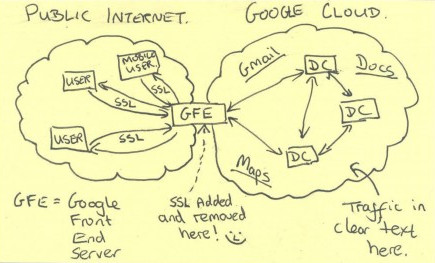
\includegraphics[width=\textwidth]{motivation.jpg}
            \caption{Government attempts to intercept user's content}
        \end{figure}
    \end{frame}
    \begin{frame}{History of VPN protocols}
        \begin{itemize}
            \item IPSEC
                \begin{itemize}
                    \item Popular for site to site connections with dedicated router hardware,
                    \item Tedious to set up and high degree of complexity,
                    \item Large attack surface between IKE (v2), SA mechanisms, XFRM in Linux,
                    \item Legacy protocol support,
                    \item IP in IP,
                \end{itemize}
            \item OpenVPN
                \begin{itemize}
                    \item Implemented in userspace with TUN/TAP (slow),
                    \item Complex confoguration vulnerable to leaks,
                    \item Stateful protocol which is brittle in real networks,
                    \item Large codebase / attack surface,
                \end{itemize}
        \end{itemize}
    \end{frame}
    \begin{frame}{What is Wireguard?}
        \begin{itemize}
            \item Opinionated Layer 3 secure network tunnel for IPv4 and IPv6.
            \item Lives in the Linux kernel, but cross platform userspace implementations are available.
            \item UDP based. Punches through firewall.
            \item Modern conservative cryptographic principles.
            \item Emphasis on simplicity and auditability.
            \item Authentication model similar to SSH's \texttt{authorized\_keys}.
        \end{itemize}
    \end{frame}
    \begin{frame}{Easily Auditable}
        \begin{figure}
            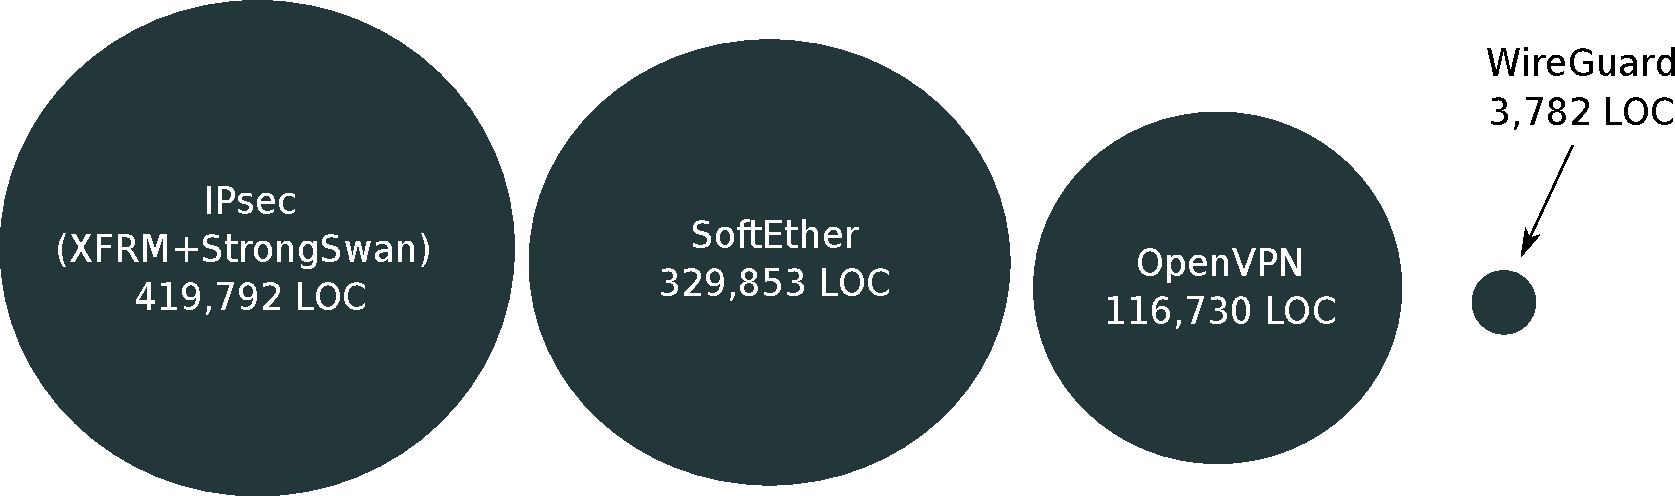
\includegraphics[width=\textwidth]{vpn_compare.pdf}
            \caption{Comparing different VPN protocols in terms of LOC}
        \end{figure}
    \end{frame}
    \begin{frame}[fragile]{Minimialistic Interface}
    ``Developers should write programs that can communicate easily with other programs''
    \\[5pt]
    \rightline{{\rm --- Unix Philosophy}}
        \begin{itemize}
            \item Wireguard presents a normal network interface
                \begin{lstlisting}
# ip link add wg0 type wireguard
# ip address add 10.0.32.1/24 dev wg0
# ip route add default via wg0
                \end{lstlisting}
            \item By using a standard interface it becomes easier to administer using the existing iproute2 utilities for example
        \end{itemize}
    \end{frame}
    \begin{frame}{Cryptokey Routing}
        \begin{itemize}
            \item Fundamental concept of any VPN service
                \begin{itemize}
                    \item Create \textbf{mapping} between \textbf{public keys of peers} and their \textbf{IPs}.
                \end{itemize}
            \item WireGuard interface has:
                \begin{itemize}
                    \item A private key
                    \item A listening UDP port
                    \item A list of peers
                \end{itemize}
            \item Peer has
                \begin{itemize}
                    \item A public key
                    \item A list of associated tunnel IPs
                    \item Optionally has an endpoint IP and port
                \end{itemize}
        \end{itemize}
    \end{frame}
    \begin{frame}[fragile]{Cryptokey Routing}
    	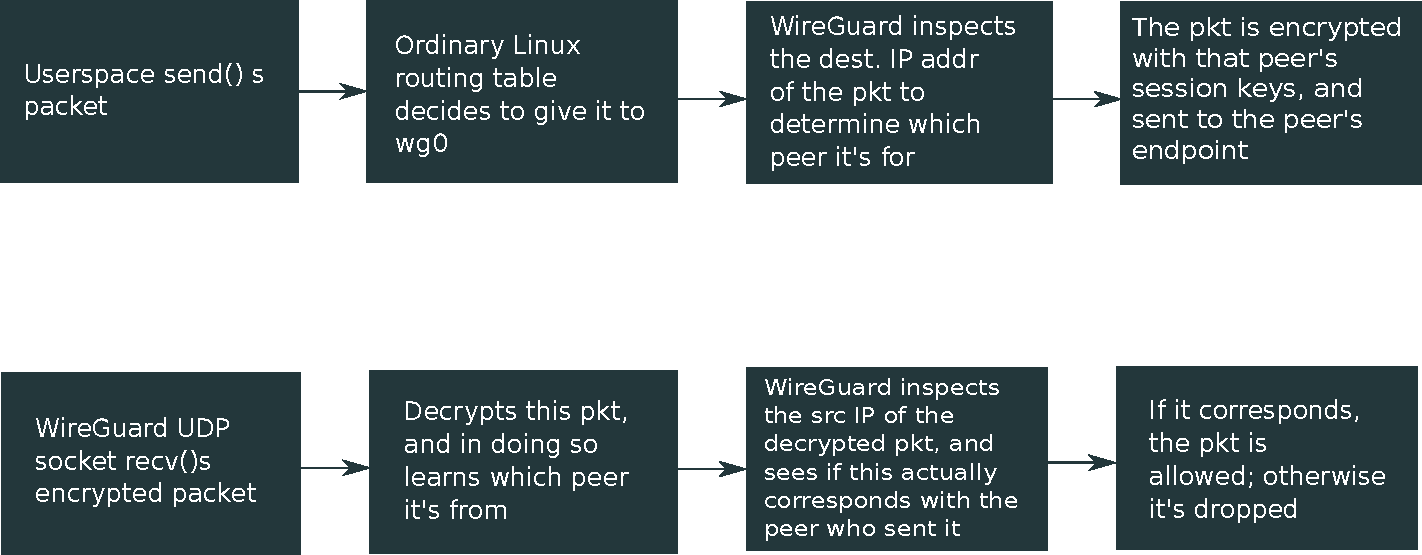
\includegraphics[width=\textwidth]{crypto_route.pdf}
    \end{frame}
    \begin{frame}[fragile]{Performance}
        \begin{figure}
            \hspace*{-1cm} \subfloat{{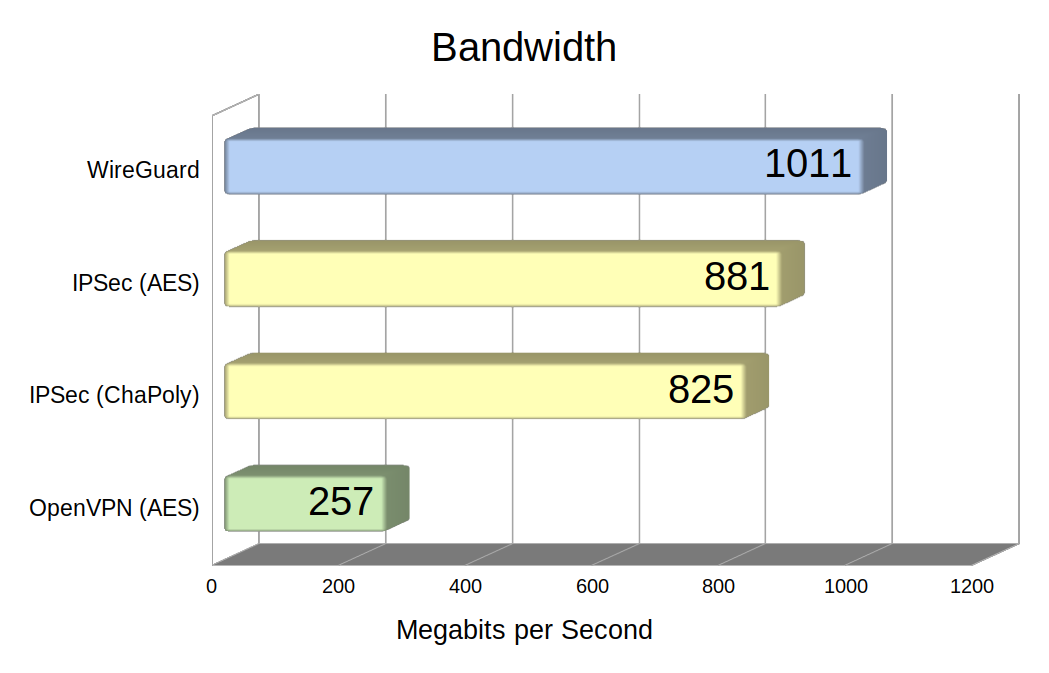
\includegraphics[width=6cm]{bandwidth.png} }}%
            \subfloat{{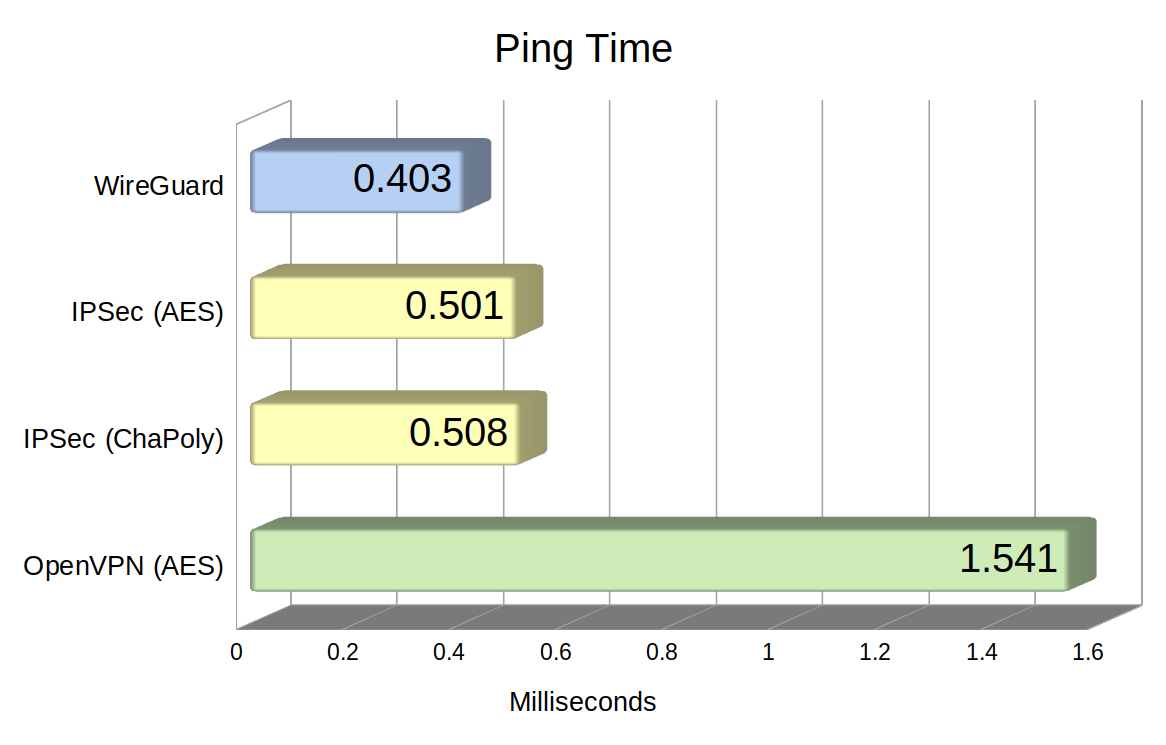
\includegraphics[width=6cm]{ping.png} }}%
            \label{fig:example}%
        \end{figure}
    \end{frame}
    \begin{frame}{Stealth}
    	\begin{minipage}{0.6\textwidth}
			\begin{itemize}
				\item Behaves like a rootkit in some sense.
				\item Should not respond to any unauthenticated packets.
				\item Hinder scanners and service discovery.
				\item Service only responds to packets with correct crypto.
				\item Not chatty at all. 
    		\end{itemize} 
		\end{minipage}
		\begin{minipage}{0.37\textwidth}
			\begin{figure}
				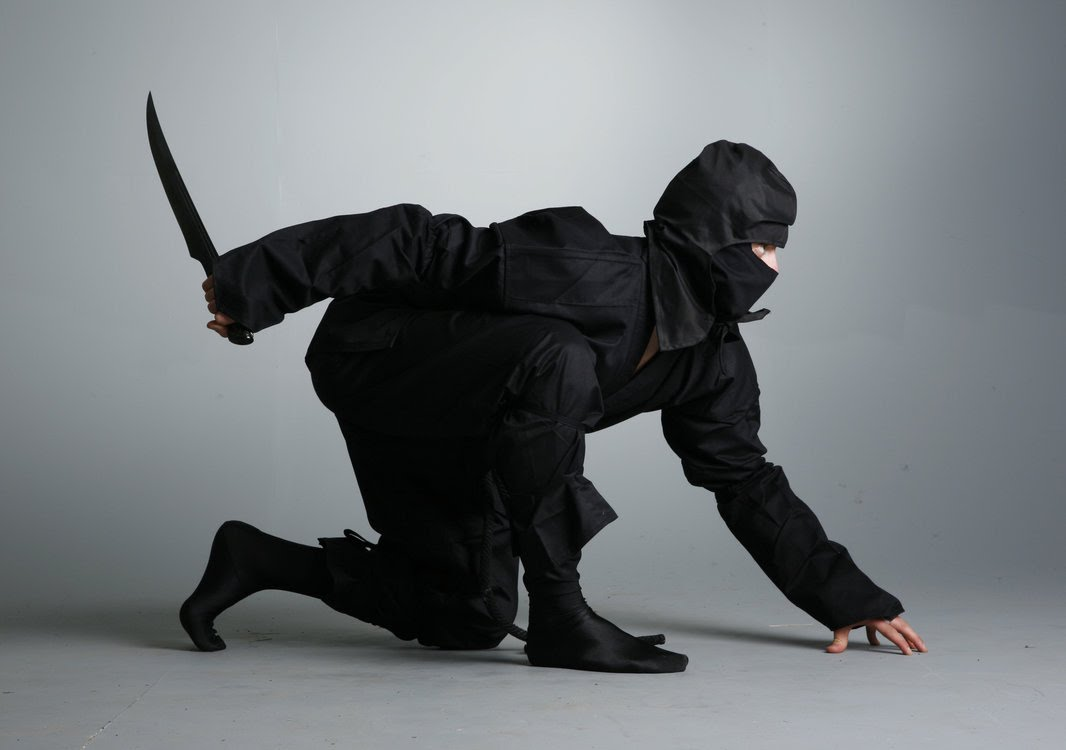
\includegraphics[width=\textwidth]{ninja.jpg}
			\end{figure}
		\end{minipage}
    \end{frame}
    \begin{frame}{The Key Exchange}
    	\begin{figure}
			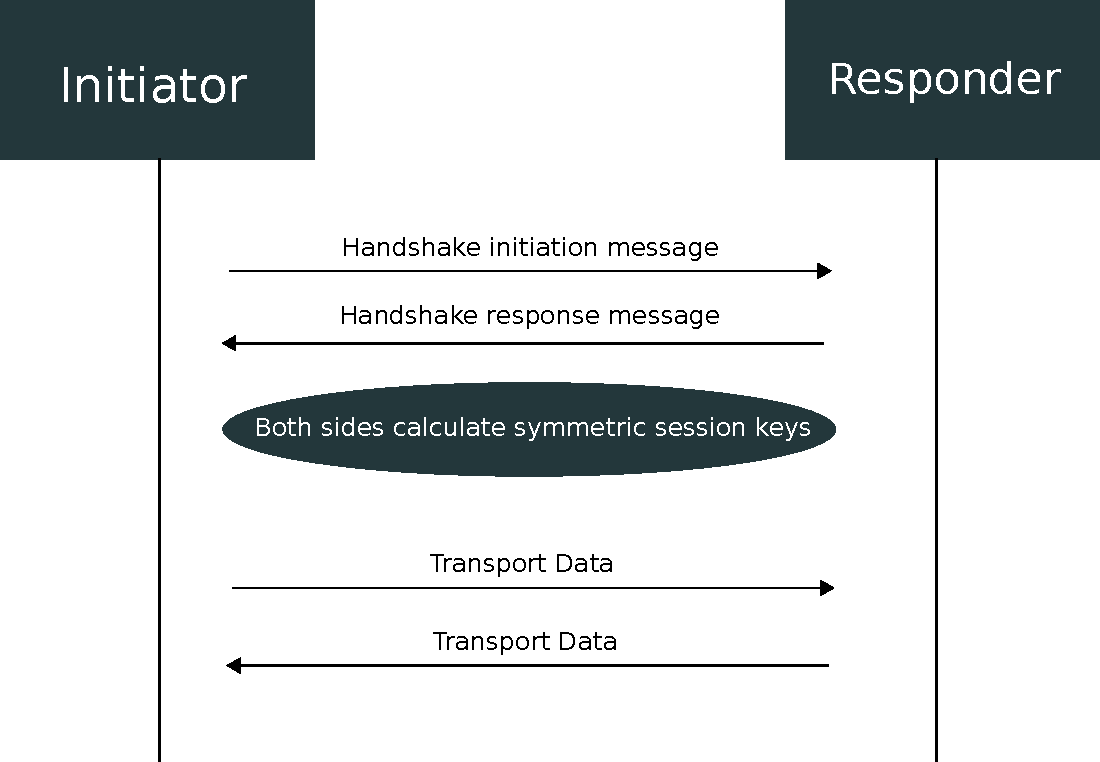
\includegraphics[width=\textwidth]{handshake.pdf}
		\end{figure}
    \end{frame}
\end{document}